%%%%%%%%%%%%%%%%%%%%%%
\documentclass{doublecol-new}
%%%%%%%%%%%%%%%%%%%%%%

\usepackage{natbib}
\usepackage{html}
\usepackage{url}

\usepackage[utf8]{inputenc}
\usepackage{lmodern}

\def\newblock{\hskip .11em plus .33em minus .07em}

\makeatletter
\def\theequation{\arabic{equation}}

\JOURNALNAME{\TEN{\it Int. J. of Systems, Control and
Communications, Vol. \theVOL, No. \theISSUE, \thePUBYEAR}\hfill\thepage}%

\def\BottomCatch{%
\vskip -10pt
\thispagestyle{empty}%
\begin{table}[b]%
\NINE\begin{tabular*}{\textwidth}{@{\extracolsep{\fill}}lcr@{}}%
\\[-12pt]
Copyright \copyright\ 2016 Inderscience Enterprises Ltd. & &%
\end{tabular*}%
\vskip -30pt%
%%\vskip -35pt%
\end{table}%
} \makeatother

%%%%%%%%%%%%%%%%%
\begin{document}%
%%%%%%%%%%%%%%%%%

\setcounter{page}{1}
\LRH{G. L. Camillo and C. M. Westphall}
\RRH{Privacy Preserving in finer grained access control using XACML and OpenID Connect}
\VOL{x}
\ISSUE{x}
\PUBYEAR{xxxx}
\BottomCatch
\CLline
\PUBYEAR{2015}

\subtitle{}

\title{\sf{\textbf{Privacy preserving in finer-grained access control using XACML and OpenID Connect}}}

\authorA{\sf{Gerson Luiz Camillo*,Carla Merkle Westphall}}

\affA{Departamento de Informática e Estatística (UFSC-CTC-INE),\\
	Universidade Federal de Santa Catarina,\\	
	Laboratório de Redes e Gerência,\\	
	CEP 88040-900 - Campus Universitário
	Florianópolis, Santa Catarina, Brasil	
	Phone: +55 048 3721-  \\
E-mail: gerson.camillo@posgrad.ufsc.br\\
E-mail: carlamw@inf.ufsc.br\\
{\sf{*}}Corresponding author}

\begin{abstract}
Muitos provedores de serviço começaram a implantar personalização em seus portais, de forma que um indivíduo agora não só apresenta a comprovação de identidade digital mas também precisa divulgar Personally Identifiable Information (PII), conhecidas como atributos no contexto do controle de acesso. A soltura (release) de PII representa um problema de privacidade. Este texto propõe um modelo que permite ao indivíduo obter serviços sem a necessidade de divulgar PII, mas apenas o resultado da política de granularidade fina sobre o valor do atributo. Também apresentamos uma implementação de um protótipo além de apresentar um caso representado um cenário hipotético para avaliação. O projeto demonstrou que para certos casos um usuário pode restringir a liberação de determinados PII ao mesmo tempo em que pode obter acesso aos serviços.
\end{abstract}

\KEYWORD{access control; XACML; federated identity management; OpenID Connect; privacy preserving.}

\REF{to this paper should be made as follows: Camillo, G.L. and Westphall, C.M.. (2015) `Privacy preserving in finer-grained access control using XACML and OpenID Connect', {\it Int. J. Security and Networks}, Vol.~x, No.~x, pp.xxx--xxx.}

\begin{bio}
Gerson Luiz Camillo received his BSc in Computer Science from the Universidade Federal de Santa Maria, RS, Brasil. His research interests include security, access control and identity management.\vs{8}

\noindent Carla Merkle Westphall is a Professor in the Departamento de Informática e Estatística of Universidade Federal de Santa Catarina (UFSC) Brazil. She is working in security since 1996. Her research interests include information security, distributed security, identity management and cloud security. She received her PhD in Electrical Engineering (Information Systems Security) from the Universidade Federal de Santa Catarina. She is a member of the Networks and Management Laboratory which has many master and doctoral students developing security research.

\end{bio}

\maketitle

\section{Introduction}

As tecnologias de autenticação e autorização tem evoluído em questões de segurança, usabilidade e performance para se adequarem ao contexto da distribuição de serviços na Web. O navegador se tornou a principal interface para consumo e apresentação de informação. Os dados que identificam e caracterizam o usuário adquiriram valor inestimável no sociedade digital de tal forma que qualquer transação na Internet na maioria das vezes requisita que a alguma informação seja liberada. 
This data is represented by attributes and is named as Personally Identifiable Information (PII). The relationship of the traces we take while navigating in Internet and the information that identify us transformou empresas em gigantes, as such Google and Yahoo.

A aplicação da privacidade possui dois contextos\cite{kagal2010access}: um está relacionado ao controle de acesso sobre como a informação se torna conhecida enquanto que o outro é como os dados são usados. O segundo 

MOTIVAÇÃO: por que é importante PRIVACIDADE.
The privacy aims to control and protect both data owns by a user and the PII proving law, techniques and mechanisms to empower the entity about its information. Specificaly, in the area of computer security, privacy qual se procura minimizar a quantidade de informação pessoal liberada e/ou impedir que atributos sejam ligados ao usuário \citep{gurses2011engineering,heurix2015taxonomy,landwehr2012privacy}. Privacy was subject a concern a long time ago. The importance of protect personal data levou às primeiras iniciativas de regulação. And the first normative was established in 1981 with guidelines to protect the privacy of personal data in EU \citep{oecd1981guidelines} with the establishment of eight principles. These principles influenced the criation of directives, laws and frameworks around the world. The importance of privacy today is reflected in the revision of the guidelines \citep{oecd2013guidelinesupdated} and the consequences in the form of companies work with personal data \citep{kuschewsky2014new}. 

POR QUE É IMPORTANTE RESOLVER O PROBLEMA: exemplos de aplicações
To realize to motivation problem we present a scenario of a library, as used in the paper of \citep{camenisch2014concepts}. The librarian do not can rent titles (books, films) to persons who age is under 18. To increment the usability, the library will send free of charge books to people who have 60 or older and who live in the centre region of the city. Considering the service will include the option of privacy preserving of user data, how we can create a solution that allows the individuals use the service without exposing personally identifiable data? This question involves two sides of service negotiation: the service provider need guarantee the restriction on using the some services and the user don't want discloses personally information.

O QUE O PRESENTE TRABALHO TEM DE INOVADOR em relação aos outros trabalhos, CONTRIBUIÇÃO:
The above problem guided the search of related works and systems that presented solutions to achieve privacy in using online services. The context of problem and the proposes of this work relates service provider (SP) enforcing fine-grained policies over personally attributes managed by an identity provider (IdP). Both are executed in disjunct security domains. Specifically, the SP runs XACML and the IdP, OpenID Connect, under Representational State Transfer (REST) services and protocols. The only paper that deals with that entities and in environment of privacy preserving was \citep{ma2015cloud}, but in that case, the entity that manages policies is in the same domain of identity provider. The privacy-preserving Attribute-based Credentials (Privacy-ABCs) technologies \cite{camenisch2009credential,dagdee2011extending} offers solution for privacy-preserving of PII robustness of underlying cryptography, but is a complex system. The User-Managed Access (UMA) profile of OAuth 2.0 \cite{hardjono-oauth-umacore-14} is solution to authorization in Web 2.0 that can be integrated to OpenID Connect bringing novel perspectives to users manage the access control. But UMA depends strongly on the user defining policies and on the resource server to enforce such policies (there is a step that establishes a trust relationship between the entities). 

We present in this paper a different approach, that permits the user minimized the personal information released to the service provider resource server while still maintaining access to resources/services. There isn't necessary to trust in the the service provider, because it trust that the user possess the required attribute. The idea has similarities with the Privacy-ABC technologies, but the proposed model is supported by recent protocols and specifications, like OAuth 2.0, OpenID Connect for identity management and RESTful as the means of transportation. Aside, the service provider applies fine-grained authorization using XACML architecture and policies.

The main contributions of this works are: apresentação de um framework para avaliar políticas de controle de acesso por atributos no provedor de identidade, retornando para o provedor de serviço somente o resultado da avaliação, objetivando impedir que o provedor de serviço obtenha dados privados do usuário; the service provider can enforce fine-grained access control policies using XAML while keeps user privacy about PII; and, presents a prototype to evaluate a use case of scenario.

The remaining of this paper is organised as follows: Section 2 presents the related works; Section 3 discusses access control, identity and privacy; in Section 4 the proposal is presented; Section 5 shows the development; the results are
presented in Sections 6 and 7 has some conclusions and the description of future works.

\section{Related works}
There are a broad range of solutions to enhancing privacy in systems that delivery services using or providing data relative to a person. The systems are known Privacy Enhancing Technologies (PET). A lot of PET and proposals have the purpose of augment or stablish privacy in the relationship between users and service providers when some form of personal data is involved. The range start with Cookie-cutters blocking cookies and language privacy of Platform for Privacy Preferences (P3P) ending with cryptographic solutions using including third-party authorities, such as the Privacy-Attribute Based Credentials (Privacy-ABC). To restrict the works to analyse and compare, we restrict to the privacy of personal data, as defined in EU Directive 95/46/EC\cite{directive199595} that refers to the piece of information that identifies directly or indirectly a natural person. As we are working on data minimization, the scopes left out the proposes that treats how data is used, according to \citep{mondal2014beyond}.

\citep{kolter2007privacy} foi um dos primeiros trabalhos que buscou resolver a questão de privacidade em sistemas de controle de acesso baseados em atributos sobre Service-oriented Architectures (SOA). O autor estendeu a plataforma XACML para suportar PDPs separados do provedor de serviço. Essa arquitetura permite que o usuário, ao acessar o serviço, defina qual sua preferência de privacidade, o que determina a escolha do PDP mais adequado. Mas isso requer que o provedor de serviço confie na decisão gerada pelo respectivo PDP. Questões de confiança no transporte de autorizações foram resolvidas através de infraestrutura de chaves públicas. Um importante conceito apresentado foi de associar diferentes PDPs a perfis de privacidade. Porém, a proposta não apresentou um protótipo e foi planejada para ser incluída no projeto Access-eGov\cite{pernulAccesseGov}, que foi proposto para ser uma plataforma de composição de serviços governamentais baseados em Web semântica.

Uma outra vertente de propostas é o controle de acesso baseado em certificados de atributos, que constituem-se em uma lista de pares atributos-valores digitalmente assinados. Duas propostas foram apresentadas dentro do projeto Privacy and Identity Management for Europe (PRIME), por \citep{ardagna2008privacy} e por \citep{ardagna2010exploiting}. Between 2008 and 2011 the work continued in the projetc Privacy and Identity Management in Europe for Life (PRIMELife) que tinha por objetivo apresentar soluções in identity management, integrating access control policy with com políticas de manipulação de dados com privacidade. The works allow individual prove the possession of condition to satisfy the restrictions imposed by services on attributes without revealing personal information. As propostas não tiveram muito sucesso prático tendo em vista as dificuldades de implementação. Além disso, certificados de atributos precisam do suporte de uma infraestrutura de chaves públicas e há questões envolvendo revogação e armazenamento dos certificados. Pelo fato de constituir o modelo de autorização do projeto PRIME, não tem sido implantado em cenários reais devido dificuldade de implementação \cite{ardagna2010enabling}.

Em vista dos problemas das propostas anteriores e também pelo fato do XACML não prover facilidades para acomodar certificados de atributos \citep{dagdee2011extending}, \citep{ardagna2010enabling} apresentou uma solução de controle de acesso baseado também em certificados de atributos mas usando padrões de mercado, no caso XACML \citep{rissanen2013extensible} e SAML \citep{ragouzis2008security}. O primeiro, para autorização baseada em atributos, enquanto o segundo como um meio de transporte de declarações sobre fatos de autenticação e/ou autorização. No artigo o autor somente apresentou o modelo, não incluindo testes de validação de um possível protótipo, considering that the implementation was occurring in PRIMELife project.

Outro trabalho \cite{kounga2010extending} também seguiu a linha de estender o XACML, mas definindo uma autoridade que armazenasse os atributos e políticas. A proposta de Kounga em \cite{kounga2010extending} aborda a possibilidade de que o consentimento do usuário pode se estender tanto nas preferências de privacidade das informações pessoais quanto em dados. Além disso, através da extensão do XACML o consentimento pode ser de granularidade mais fina sobre os dados. Para evitar que os pontos PDP e PEP do XACML não tenham acesso às preferências de privacidade e de dados do usuário a arquitetura foi estendida para incluir módulos que tratam exclusivamente dos dados de atributos, que foi definido como \textit{Attribute Authority} (AA). Apesar de apresentar a característica de autorização com privacidade, a solução necessita que uma autoridade de confiança (chamada de \textit{data collector}) gerencie as preferências e os dados pessoais. Além disso, o artigo não apresentou uma implementação da proposta, em parte, devido ao fato da solução usar alguns conceitos e estender o \textit{framework} do projeto \textit{Identity Governance Framework} (IGF). A extensão do XACML para acomodar controle de acesso baseado em certificados de atributos foi explorada pelos trabalhos de \citep{camenisch2009credential} e \citep{dagdee2011extending}, o primeiro na forma de uma linguagem e outro na extensão da arquitetura.

Chadwick propôs uma arquitetura em \cite{chadwick2012privacy} que fornece serviço de autorização para ambiente em nuvem. A questão de privacidade é tratada sob dois aspectos: primeiro, através de diferentes PDPs que avaliam cada qual uma linguagem de política de privacidade diferente; e o conceito de \textit{sticky policy}, que permite que os dados trafeguem entre instalações de nuvens mas mantendo presa a política de privacidade. O pressuposto adotado no trabalho foi que os provedores de serviço na nuvem são confiáveis de tal forma que vão honrar as políticas de privacidade definidas nas sticky policies oriundas de outros provedores no mesmo ambiente de nuvem. Trata-se de proposta dentro do projeto PERMIS \cite{chadwick2008permis} that is framework to provide policy based authorisation for federated and/or grid applications using the standard SOAP/SAML protocol. The goal of the project is create a system with privacy preserving authorization and tools for management of policies. The architecture was defined and constructed over the SAML protocol and the entity that provide de user data was not specified by \cite{chadwick2012privacy} but PERMIS can be integrated with Shibboleth and Globus toolkit, while our proposal uses RESTful and OpenID Connect. Although the user has control of his privacy PII, the model depends on the service provider respect the policy.

Architectures for policy decomposition \cite{lin2008policy} and policy federation \cite{decat2012toward,decat2013federated,decat2014middleware} aimed to provide confidentiality and privacy when enforcing access control policies in distributed environment. The proposed works are supported by the XACML policy and architecture, because the entities are specified to be easy distributed. The proposed works are supported by SOAP/SAML protocols and the relationship with identity providers were not defined in their proposals. 

The Privacy-ABC technologies are proven solutions to create solutions for privacy preserving PII. There are based in cryptography a important 
Sistemas de gerenciamento de identidade baseados em credenciais foram propostos, valendo destacar o IDEMIX\cite{camenisch2002design}, sistema da IBM, baseado no esquema de Camenisch-LysyansKaya \cite{camenisch2001efficient} e o U-Prove, especificação criada por \cite{brands2000rethinking}, atualmente pertencente à \textit{Microsoft}. O primeiro foi criado a partir de primitivas criptográficas e é baseado em credenciais anônimas para permitir transferência de atributos de forma a manter privacidade. Os dois sistemas acabaram virando sistemas empresariais e a complexidade dos mesmos é alta \cite{nogueira2014aprimoramento}.

O trabalho de \cite{ma2015cloud} apresentou um modelo em que os usuários eram identificados por uma federação \textit{OpenID Connect} e o controle de acesso através do XACML. Para incluir o consentimento dos usuários sobre a liberação de seus dados, foi criado um servidor de políticas XACML ligado ao servidor de identidade. Apesar de usar padrões atuais, a solução de Ma foi adaptada especificamente para resolver a questão do acesso de pacientes, médicos e colaboradores sobre os dados de imagens de diagnóstico médico disponibilizados por diferentes clínicas e hospitais dentro de uma nuvem.

O trabalho que mais se aproxima da proposta do presente projeto é o que Ma apresentou em \cite{ma2015cloud}, pelos seguintes motivos: usa padrões atuais, o \textit{OpenID Connect} para solução de federação de identidade e XACML para controle de acesso de granularidade fina. Tendo em vista que a proposta foi desenhada para controlar o acesso de pacientes, médicos e pesquisados a dados de diagnósticos por imagens, foi incluída a necessidade de diretivas de consentimento para regular com melhor granularidade as condições para acesso aos dados de imagem. O mérito da proposta é a inclusão de um servidor de políticas XACML ligado ao servidor de identidade \textit{OpenID Connect}. Essa solução permitiu descrever os escopos e atributos mais complexos em termos de linguagem de controle de acesso do XACML.


O \textit{Shibboleth} é uma infraestrutura para criação de federações de identidade e tendo sido implementado sobre o protocolo SAML. O uso mais difundido tem se dado dentro da comunidade acadêmica, possuindo instalações em diversos continentes. O SAML que serve de base para a federação \textit{Shibboleth} permite o transporte de informações de atributos do usuários do provedor de identidade para o recurso. Os provedores de serviço são definidos pelo \textit{Shibboleth}, de forma que não permitem políticas de controle de acesso mais avançadas, além do fato de não estarem baseadas em padrões estabelecidos.

Outra solução que implementa federação de identidade é o \textit{OpenID Connect}, que é uma especificação de uma camada de identidade sobre o protocolo de autorização OAuth versão 2.0. Possui suporte à liberação de atributos para provedores de serviço por parte do usuário através de consentimento. O transporte de \textit{tokens} de autorização no formato JSON ocorre sobre mensagens REST. A vantagem é a possibilidade de criar clientes mais leves para dispositivos móveis.




\subsection{Tabela comparativa}

Para localizar a prosposta apresentada no presente projeto, foram apresentados na \ref{tab-tabela-comparativa} as principais características dos sistemas.

\begin{table}
	% \begin{table}[h]
	\tiny
	\centering
	\caption{Tabela comparativa entre as principais características referentes aos trabalhos relacionados.}
	\label{tab-tabela-comparativa}
	\begin{tabular}{|m{8em}|c|c|c|c|c|c|c|c|c|}
		\hline  & GerenIdent & \textit{AuthZ}(fina/grossa) & \textit{AuthZ}(modelo) & PadrõesMercado & Protótipo & ImplemVincProjeto & Complexidade \\ 
		\hline \cite{kolter2007privacy}     & Não        & Fina   & XACML           & Não            & Não(Access e-Gov) & Sim(Access e-Gov) & S/I \\ 
		\hline \cite{ardagna2008privacy}    & Sim(PRIME) & Grossa & Privada         & Parcial        & Sim               & Sim(PRIME)        & Alta(1) \\ 
		\hline \cite{ardagna2010exploiting} & Sim(PRIME) & Grossa & Privada         & Parcial        & Sim               & Sim(PRIME)        & Alta(1) \\ 
		\hline \cite{ardagna2010enabling}   & Não        & Fina   & XACML           & Sim(XACML,SAML)  & Não               & Sim(PrimeLife)    & S/I \\ 
		\hline \cite{kounga2010extending}   & Não        & Fina   & XACML           & Sim            & Não               & Sim(IGF)          & S/I \\ 
		\hline \cite{chadwick2012privacy}   & Não        & Fina   & XACML           & Parcial        & Sim               & Sim(PERMIS)       & Baixa(2) \\ 
		\hline \cite{ma2015cloud}           & Não        & Fina   & XACML           & Sim            & Sim               & Sim               & Baixa \\ 
		\hline \textit{Shibbolet}           & Sim        & Grossa & Privado         & Sim(SAML)      & Sistema em produção & \-     & Baixa/média \\
		\hline \textit{OpenID Connect}      & Sim        & Grossa & OAuth 2.0       & Sim(OAuth2.0)  & Sistema em produção & \-     & Baixa \\    
		\hline Proposta                     & Sim        & Fina   & XACML           & Sim            & Sim               & Baixa             & Sim(3) \\
		\hline 
	\end{tabular} 
	\\ Fonte: o autor.
	\\ Observações: S/I sem informações.
	\\ (1): complexidade conforme definido em \cite{nogueira2014aprimoramento}.
	\\ (2): complexidade de execução baixa conforme resultados no artigo \cite{chadwick2012privacy}.
	\\ (3): expectativa considerando os protocolos e sistemas usados pela proposta.
	% \end{table}
\end{table}

Detalhamento dos aspectos analisados nas propostas:
\begin{enumerate}
	\item A
	\item Gerenciamento de Identidade: verifica se a proposta inclui o relacionamento com um sistema de gerenciamento de identidade, ou seja, se há alguma sistema que fornece os atributos para autorização.
	\item Autorização (\textit{AuthZ}) (fina/grossa): especifica se a autorização é considerada sobre os atributos individuais do sujeito, recurso e ambiente, consistente com o modelo ABAC, o qual determina a autorização de granularidade fina. Caso contrário, diz-se que o sistema implementa autorização de granularidade grossa.
	\item Autorização (modelo): quando a proposta define um sistema de autorização, verifica se a mesma se baseia em algum modelo ou é proprietário à proposta.
	\item Padrões de mercado: algumas propostas podem fazer uso ou estender padrões ou especificações de mercado para mecanismos de controle de acesso, autorização e transporte de mensagens. As especificações mais adotadas nesse ramos de estudos são: XACML, SAML, OAuth, OpenID e \textit{OpenID Connect}.
	\item Protótipo: se foi ou não criado um protótipo com alguns resultados de validação.
	\item Implementação vinculada à projeto: alguns artigos apresentaram propostas dentro de projetos aos quais estavam vinculados. Um aspecto negativo desses artigos é que muitas suposições e contextos estão vinculados às definições dos projetos e/ou sistemas, dificultando ao pesquisador obter e testar as propostas
	\item Complexidade: essa característica está ligada tanto à implantação da proposta quanto à complexidade de execução.
\end{enumerate}


\section{Background and Context}
This section discusses the main topics that are related to the context of this work. Specifically, access control, identity management and privacy.

The access control is the center of security of any information asset resides A segurança em sistemas computacionais têm por objetivo proteger recursos que possuem algum valor para o detentor dos mesmos. Os ativos de informação possuem basicamente três propriedades de segurança \cite{gollmann2011compsecurity}: confidencialidade, integridade e disponibilidade. Outras características também podem ser priorizadas, como autenticidade, contabilidade (em inglês, \textit{accountability}) e não-repúdio. 

A privacidade pode ser obtida quando se aplica a propriedade da confidencialidade especificamente sobre dados pessoais. Como será detalhado mais adiante, os dados pessoais podem conter classificações mais precisas, como aquela definida em \cite{heurix2015taxonomy}.

Mais especificamente, adotando a definição de  \cite{gollmann2011compsecurity}, segurança em computação é aquela que trata da prevenção e detecção de ações não autorizadas por usuários de um sistema computacional. A definição subsidia a importância dos mecanismos de controle de acesso. O controle de acesso é o centro de gravidade de um sistema computacional e é onde a engenharia de segurança encontra a ciência da computação sendo empregada em todos os níveis computacionais, desde o \textit{hardware} até o nível de aplicativo \cite{anderson2008security}.

Tradicionalmente, o controle de acesso consiste de duas etapas: a autenticação e a autorização \cite{gollmann2011compsecurity}. A autenticação é o mecanismo que provê meios de verificar corretamente a identidade do principal\footnote{O termo principal se refere à entidade (humano, processo, máquina, etc) que interage com um sistema computacional. Esse termo foi melhor caracterizado no tema da segurança de sistemas operacionais \cite{gollmann2011compsecurity}. O presente texto adotará intercambialmente os termos principal, sujeito e usuário.} Ela é realizada em duas fases: a primeira, que é a identificação, no qual um principal apresenta uma afirmação (em inglês, \textit{claim\footnote{Pedaço de informação declarando algo sobre uma entidade. Será mantida a versão em inglês do termo no texto.}}) sobre quem é, o que pode ser um nome; e a segunda, trata de verificar se a afirmação corresponde ao principal, processo conhecido como autenticação. 

A função da autorização é definir qual principal está assegurado o acesso a que recurso do sistema. A evolução dos modelos de controle de acesso e a disseminação da computação distribuída através da Internet permitiu categorizar the Identity-Based Access Control (IBAC) e os de controle de acesso em ambientes computacionais abertos \cite{gollmann2011compsecurity}.

Sistemas de controle de acesso baseados em identidade assumem que a autenticação foi realizada e o principal foi identificado com sucesso. Os três sistemas clássicos de ampla adoção e que são baseados no princípio mencionado são: the Discretionary Access Control (DAC); the Mandatory Access Control (MAC); e o mais recente, the Role Based Access Control (RBAC).

O controle de acesso discricionário \cite{lampson1974protection} se baseia em uma matriz de acesso constituída de domínios de proteção (usuários e objetos) cuja principal característica é o fato deste modelo delegar a política de segurança para o usuário, ou seja, as entidades controlam quem e como pode realizar determinado acesso. Possui ampla adoção, resultado de sua simplicidade e flexibilidade. O controle de acesso mandatório tem por base a classificação dos sujeitos e dos objetos no sistema. Cada usuário e cada objeto possui um nível de segurança, vindo esses sistemas também serem denominados de Multilevel Security (MLS). Como exposto por \cite{sandhu1994access}, o nível de segurança associado ao objeto reflete a sensibilidade da informação contida no mesmo, ou o potencial de dano caso haja vazamento da respectiva informação, enquanto que o nível de segurança associado ao usuário, também chamado de level of clearance, reflete a confiabilidade do usuário em não divulgar informação. 

O modelo que foi proposto a seguir foi o Role-Based Access Control (RBAC), que foi formalizado por \cite{ferraiolo1992role} e cuja principal motivação foi atender ao estabelecimento de políticas de controle de acesso em ambientes corporativos. A característica principal deste modelo é a separação da ligação direta entre os usuários e as respectivas permissões. Aos papeis são associados conjuntos de permissões que regulam as operações sobre os objetos. Os usuários são então associados a determinados papeis, e os mesmos podem ativar o subconjunto dos mesmos, determinando o conceito de sessões. Os princípios de segurança mais importantes suportados pelo RBAC são os seguintes, conforme encontrado em \cite{sandhu1996role}: o primeiro é o privilégio mínimo para acesso, que no RBAC pode ser configurado para que somente aquelas permissões mínimas sejam atribuídas ao papel para realização de certa tarefa; e, the Separation of Duties (SoD): cuja finalidade é evitar conflitos de interesse entre diferentes roles atribuídos aos usuários.

A evolução da computação trouxe questões que modelos tradicionais de controle de acesso baseados em identidade já não podiam satisfazer. As mais importantes foram: o usuário já não está mais definido; a computação agora é realizada tanto no servidor quanto no cliente; políticas de controle de acesso evoluíram para considerar aspectos tanto do sujeito quanto do objeto e questões ambientais relativas às operações. Essa e outras necessidades levaram à formalização of model Attribute Based Access Control (ABAC), definido formalmente em \cite{huABAC2014guide}: o controle de acesso aos objetos é obtido pela avaliação de regras considerando os atributos das entidades (sujeito e objeto), das operações e do ambiente, relevantes para a requisição. O modelo conta com várias entidades, que realizam diferente funções, permitindo a implementação distribuídos desses unidades. A definição das principais entidades e suas funções já haviam sido publicadas na Recomendação X.812 da ITU-T, de 1995, conforme publicação em \cite{itut1996acframework}. As entidades e suas função estão discriminadas a seguir:

\begin{enumerate}
	\item Policy Administration Point (PAP): entidade que cria a política;
	\item Policy Decision Point (PDP): avalia a política aplicável à requisição que resulta em uma decisão de autorização, que é retornada para a entidade responsável por cumprir a política;
	\item Policy Enforcement Point (PEP): é a entidade que efetivamente realiza o controle de acesso, protegendo o recurso. Recebe as requisições de acesso e as envia para o PDP para avaliação cujas respostas de autorização definem o cumprimento da política.
	\item Policy Information Point (PIP): serve como repositório e origem para os atributos necessários à avaliação da política.
\end{enumerate}


Serão apresentados conceitos de controle de acesso, detalhando o modelo Attribute Based Access Control (ABAC)\cite{huABAC2014guide} e a especificação eXtensible Access Control Markup Language (XACML)\cite{rissanen2013extensible}, a seguir o conceito de gerenciamento de identidade, especificamente o OpenID Connect e o conceito de privacidade.


O ABAC possui vantagens bem definidas quando se trata de usar e aplicar um sistema de controle de acesso em ambientes computacionais atuais: 

\begin{enumerate}
	\item O controle de acesso pode ser externo às aplicações, ou seja, não há uma necessidade de cada aplicação criar e manter código de autorização e de política de controle de acesso. Conceitualmente é o desacoplamento entre a lógica do negócio da lógica da autorização.
	\item Controle de acesso de granularidade fina (em inglês, \textit{fine-grained}) que permite modelar políticas de acesso considerando determinados atributos, o que quer dizer que não só importa quem o usuário é, mas sobre o que, quando, onde, porque e como.
	\item Possibilidade de incluir atributos de contexto da solicitação de acesso, como a localização do usuário requisitante. Essa característica, aliada ao fato do sujeito não precisar ser conhecido antes da respectiva solicitação, permite que esse modelo possa ser usado em Service-Oriented Architecture (SOA).
	\item O ABAC é melhor adaptado para ambientes dinâmicos do que o RBAC \cite{yuan2005attributed} \cite{huABAC2014guide}.
	\item O ABAC possui a capacidade intrínseca para autorização que incorpore informação de contexto, como hora do dia, canal usado para requisição, propósito de uso, localização do usuário.
\end{enumerate}
Ao lado das muitas vantagens, há alguns problemas, dois dos quais serão apresentados pela sua importância: o primeiro é que todos os participantes na autorização ABAC devem concordar com o significado dos atributos \cite{karp2010abac} \cite{Rubio-Medrano2015federated} e também há necessidade de definir os atributos relevantes para o controle de acesso; e, em segundo lugar, the Policy Enforcement of Policy devem ser implementados em todos os recursos que deverão ser protegidos pelo ABAC. Mas as vantagens do ABAC para serviços Web levaram à criação de uma especificação baseada em XML para expressar políticas de segurança, que ficou conhecida como XACML.

A important aspect related to authorization is the fact that for a correct decision, the entity must have all the relevant attributes required by the policy.

\subsection{XACML}
We definite Policy Based Access Control (PBAC) 
The eXtensible Access Control Markup Language (XACML)\cite{rissanen2013extensible} é uma especifição criada pelo consórcio Organization for the Advancement of Structured Information Standards (OASIS) para escrever e gerenciar políticas de segurança. A padronização vem pelo fato de empregar uma extensão do XML para criar essa linguagem. O XACML descreve tanto uma linguagem para políticas de controle de acesso quanto a arquitetura para cumprir essas políticas.

O modelo de fluxo de dados apresentado na figura fig-xacml-modelofluxodados mostra as diversas entidades do modelo e a sequência de passos desde o recebimento de uma requisição de serviço até o cumprimento da decisão.

FIGURA: modelo de fluxo de dados
	
Basicamente o modelo opera da seguinte forma. A entidade PAP é responsável por criar e manter as políticas e disponibilizá-las para o PDP. Uma requisição de acesso é feita para o PEP que a encaminha à entidade \textit{Context Handler} no formato nativo. Esta por sua vez, converte em uma requisição no formato XACML e a envia para o PDP. O PDP faz uma busca pela política e se, para avaliá-la faltarem atributos, os mesmos serão buscados nos pontos de informação de atributos através da entidade PIP. Ao terminar de avaliar uma política, a resposta é devolvida para o \textit{Context Handler} que a devolve para o PEP para o cumprimento da mesma.
	
As políticas XACML estão definidas em forma de componentes, sendo a de nível superior a \textit{PolicySet}, que pode conter outra \textit{PolicySet} ou uma \textit{Policy}. \textit{Policies} contem \textit{Rul}es, a unidade mais elementar. Uma \textit{Rule} possui os seguintes componentes: \textit{Target}, \textit{Condition}, \textit{Effect}, expressões de \textit{Obligation} e expressões \textit{Advice}.
	
A avaliação de uma política pelo PDP funciona basicamente da seguinte forma: ponto de avaliação verifica se correspondências definidas pela \textit{Target} são satisfeitas pelos atributos na requisição. Portanto, uma decisão de acesso é baseada nos atributos do sujeito, objeto, ambiente e nas operações matemáticas sobre os mesmos, os quais definem os predicados de autorização. As \textit{obligations} são ações definidas para serem executadas em conjunto com a aplicação da política.
	
A especificação XACML está em sua versão 3.0, lançada em 22 de janeiro de 2013, e conta com um conjunto de \textit{profiles} que permitem acrescentar características à especificação padrão. Alguns \textit{profiles}: política de privacidade (XACML v3.0 Privacy Policy); SAML; profile para o modelo de controle de acesso baseado em papeis (XACML v3.0 Core and Hierarchical Role Based Access Control (RBAC) Profile Version 1.0).
	
Alguns dos pontos positivos da arquitetura XACML são: separação do ponto de decisão do ponto do uso (PEP), o que permite que diversos serviços possuam pontos de execução obtendo as respostas das avaliações de um ponto central (PDP); a expressão da política em XML permite que um mesmo conjunto de políticas possa ser usado por diversos serviços.
	
Por outro lado, há questões afetam as implementações do XACML. Uma é a questão do custo de computação para analisar, extrair e escrever dados em XML, procurar atributos faltantes e para avaliar a própria lógica das políticas \cite{gollmann2011compsecurity}. Outro aspecto diz respeito à questão da privacidade dos usuários, pois o PDP, ao avaliar uma política necessita de atributos do requerente que, em última análise representam informações de identificação privativa do sujeito. Liberar atributos para a o mecanismo de avaliação de política (PDP) é um aspecto que está relacionado ao próprio modelo ABAC. Dentre algumas soluções, uma delas provê uma negociação de confiança e outra é adotar a política do privilégio mínimo, ou seja, liberar o conjunto de atributos mínimos para obtenção do serviço.
	
	
\section{Federated Identity Management}\label{sec:gerenciamento-identidades}
	
Identidade completa de um indivíduo é o conjunto de identidades parciais que representam a pessoa num determinado contexto as quais são caracterizadas por um subconjunto de valores de atributos \cite{pfitzmann2010terminology}. Por essa definição se pode concluir que uma determinada pessoa pode estar associada a mais de uma identidade, da mesma forma que no mundo real possuímos uma carteira contendo a licença para dirigir e um cartão de acesso ao local de trabalho. Cada qual possui um conjunto de atributos que foram ligados à identidade através de uma autoridade.

	
O processo de autenticar um usuário consiste em determinar a identidade do sujeito. Para minimizar a necessidade de cadastro das informações pessoais em cada provedor de serviço, surgiram os sistemas de gerenciamento de identidade \cite{el2007survey} \cite{cao2010survey}. A principal função desses serviços é habilitar o Single Sign On (SSO), de forma que o usuário realize uma única autenticação e assim tem-se acesso a diversos recursos. Conforme definido em \cite{bertino2011identity}, o Identity Management (IdM) tem por função manter a integridade das identidades através do ciclo de vida, que consta de criação, uso, atualização e revogação. 

The main objetive of IDM is securely transport attributes between parties.

O objetivo é que as identidades e os dados relacionados sejam transmitidos para os provedores de serviço de forma segura e com proteção à privacidade. Para realizar as funções de criação, gerenciamento e uso de identidades digitais, o gerenciamento de identidade deve estar suportado por um conjunto de processos e tecnologias \cite{cao2010survey}.
	
O servidor que realiza o cadastro, gerencia e disponibiliza informações de identidade para autenticação é conhecido como Identity Provider (IdP). A entidade que provê serviço mas que impõe a identificação do requerente é conhecida como Service Provider (SP). Uma federação de identidade define e regula o relacionamento entre diferentes provedores de identidade e provedores de serviço de diferentes domínios criando um único domínio virtual \cite{perez2014identity} \cite{cao2010survey}. Mais especificamente, o modelo federativo deve compreender um conjunto de acordos, padrões e tecnologias que permitam que provedores de serviço reconheçam as identidades dos usuários de provedores de identidade \cite{torres2013survey}.
	
In general the term federated represent a loosely coupled set of entities cooperating to achieve a common result.
Federated ID, also called Federated Identity Management (FIM), allows a Service Provider (SP) to offer a service without implementing its own authentication system, and to instead trust another entity—an Identity Provider (IdP)—to provide authenticated users to them.
Federated Identity is where one entity trusts another entity with user management.
	
	Vantagens de uma federação de identidade:
	- O SP não se preocupa com questões de autenticação; apenas em oferecer serviços;
	- Um única credencial para diversos serviços; e
	- SSO
	
	
Os padrões que são usados para criar sistemas de gerenciamento de identidade e federações de identidade na \textit{Web} são:  SAML, OAuth, OpenID, OpenID Connect e especificações WS-*. O padrão Security Assertion Markup Language (SAML) \cite{ragouzis2008security}, define declarações de autenticação e autorização em linguagem XML e também os protocolos de transporte dessas declarações. Vários sistemas de federações de identidade são baseadas no SAML, dos quais vale destacar o Shibboleth \cite{erdos2002shibboleth} e SimpleSALMLphp. Os protocolos OpenID\cite{openid2015} e OAuth\cite{hardt2012oauth} são baseados em HTTP e são usados para autenticação e/ou autorização de usuários sem a necessidade de divulgar credenciais (principalmente senhas) para os provedores de serviço. O OpenID foi originalmente especificado para prover autenticação enquanto que o OAuth foi criado para delegar autorização, entre SP e IdP. O OpenID Connect v. 1.0 \cite{sakimura2014openidconnect} é um procolo que estabeleceu uma camada de identidade federativa sobre o protocolo OAuth 2.0, que permite criar federações de identidade usando mensagens REST, resultando em clientes que podem ser executados tanto sobre navegadores quanto sobre dispositivos móveis. \textit{WS-Federation} \cite{goodner2009ws} é uma especificação criada pela OASIS e indústria (IBM e Microsoft) e que define os mecanismos para criar federações de identidade usando XML, mensagens SOAP e Web Services Description Language (WSDL). Ela está suportada nos padrões OASIS WS-Security e WS-Trust.
	
	
\subsection{\textit{OpenID Connect}}
	
O \textit{OpenID Connect} consiste de uma camada de identidade sobre o protocolo OAuth 2.0 que provê a funcionalidade de autenticação usando o OAuth 2.0 e o transporte de \textit{claims} sobre o usuário final para a entidade provedora de serviço. Apesar do protocolo OAuth versão 2.0 ter sido na RFC 6749 em outubro de 2012, o \textit{OpenID Connect} é uma especificação muito recente, de fevereiro de 2014. O reflexo foi o uso de fluxo de mensagens no padrão REST/JSON. Conforme o sítio do OpenID, companhias importantes já começaram o uso do OpenID Connect: \textit{Google}, \textit{Microsoft}, \textit{Ping Identity}, \textit{Deutsche Telekom}, \textit{Salesforce.com} e o Instituto de Pesquisa Nomura do Japão.
	
Na figura fig-openidconnect-fluxomensagens são apresentados os fluxos de mensagens entre as três seguintes entidades:
	
\begin{enumerate}
	\item Relaying Party (RP): entidade que requer a autenticação e afirmações do usuário final a partir do provedor de identidade OpenID Connect. A nomenclatura segue o estabelecido no protocolo OAuth 2.0, no qual essa entidade recebe o nome de cliente.
	\item OpenID Provider (OP): é a entidade capaz de autenticar o usuário final e prover afirmativas sobre o mesmo para o RP. No protocolo OAuth 2.0 é denominado de servidor de autorização (OAuth 2.0 \textit{Authorization Server}).
	\item End-User: é o usuário final, ou seja, é o ser humano participante do protocolo.
\end{enumerate}
		
FIGURA: fluxo mensagens OpenID Connect
			
Basicamente, o fluxo de mensagens seguem os seguintes passos:
\begin{enumerate}
	\item The RP (Client) envia uma requisição de autenticação para o OP (OpenID \textit{Provider}).
	\item O OP autentica (AuthN) o usuário final e obtém autorização (AuthZ).
	\item O OP responde com um Token de ID e usualmente com um Token de acesso (AuthN \textit{response}).
	\item O RP pode enviar a requisição contendo o Token de acesso para o ponto de informação sobre dados (atributos) do usuário (\textit{UserInfo Endpoint}).
	\item O ponto de informação (\textit{UserInfo Endpoint}) retorna \textit{claims} sobre o usuário final.
\end{enumerate}
				
Sobre o fluxo, há algumas considerações. As mensagens iniciam com o usuário fazendo uma requisição de acesso a uma aplicação no lado do RP. As mensagens (1), (3), (4) e (5), no fluxo padrão, são redirecionadas através do usuário, geralmente via navegador \textit{Web}.

\section{Privacidade}

A privacidade é um conceito amplamente divulgado mas que não possui uma definição única. Para este trabalho será adotado os autores \cite{pfitzmann2010terminology} propõem ampla conceituação envolvendo esse tema. Primeiramente, privacidade é o direito de indivíduos, grupos ou instituições de determinar quando, como e qual informação sobre os mesmos é comunicada aos outros. Ainda, traz o importante conceito de minimização de dados, o qual resumidamente é diminuir a possibilidade, a quantidade e o tempo sob guarda de dados pessoais por terceiros. Dos objetivos relacionados à privacidade e minimização de dados, conforme encontrados em \cite{pfitzmann2010terminology} e \cite{deng2011privacy}, três serão apresentados a seguir, por serem importantes no presente trabalho:
\begin{enumerate}
	\item Anonymous: diz-se do sujeito que não é possível ser identificado dentro do conjunto;
	\item \textit{Unlinkability}\footnote{Será mantida a palavra em inglês durante o texto.}: propriedade na qual dois ou mais itens (atributos ou ações) do sujeito não podem ser ligados entre si e/ou associados a um sujeito; e
	\item \textit{Undetectability}\footnote{Ibidem.}: capacidade de um sistema ocultar itens ou transações relativas a um sujeito.
\end{enumerate}

Uma linha importante que estende sistemas de controle de acesso para prover privacidade é a inclusão do atributo purpose que representa a finalidade para determinado acesso (ou para qual fim uma informação é usada) e que deve ser determinado pelo sistema antes da respectiva requisição. O texto de \cite{byun2005purpose} apresenta um modelo de controle de acesso baseado numa extensão do RBAC que incorpora atributos com propósito nos papeis e papeis condicionais.

The principal norm of privacy aim to balance of data usage and the protection of personal data.

\cite{kuschewsky2014new}
Legal context
In 1980, the OECD adopted a set of eight basic privacy principles. Today, these principles are reflected in all relevant general data protection frameworks worldwide, including the EU’s Data Protection Directive 95/46/EC, the EU-US Safe Harbour framework and the APEC Privacy Framework. The OECD’s Guidelines governing the protection of privacy and transborder flows of
personal data (hereafter ‘1980 Guidelines’) is one of the earliest initiatives in the area of data protection at inter-
national level. However, in contrast to the Convention for the Protection of Individuals with Regard to the Automatic Processing of Personal Data (‘Convention 108’), 3 adopted by the Council of Europe in 1981, the Guidelines are not legally binding. The Guidelines aimed to address two different concerns, namely the risk for the privacy of individuals arising from the increased use of personal data and the risks for the free flow of information across borders due to disparate national data protection legislation. Since the 1980s the volume of personal data has increased exponentially. New technologies facilitate the storage, processing and sharing of personal data, and this at global level, and enable organizations to monitor the geolocation, activities and behaviour of individuals, thus elevating concerns regarding the implications for individuals’ privacy. In light of these technological developments and challenges, several existing data protection frameworks are being refined, including the EU’s Data Protection Directive, and more and more countries adopt data protection legislation. Today, there are more than 90 countries in six continents with data protection laws and the number is going to increase with countries like Brazil, China and India working on new laws. All these changes have led to the revision of the 1980 Guidelines.


\section{Example Scenario}

In this section we will illustrate the problem and the proposed solution through a sample scenario. The example refers to a public library (PubLib) that permits borrowing materials like books and digital media to a citizens that have been registered in an public organization (PubOrgIdP) that supports an identity provider. The library don't want maintain system and/or database of the users profile.

The library wants use authorization based on attributes and externalized of the application. The service should run on RESTful architecture, that permits the use of service by desktop/mobile platforms. The solution that permits comply with the requirements is the XACML 3.0, because is modular, have included the REST/JSON profiles and the policy of use of service can be enforce by specifying the rules in the language. The organization that offers service of identity provider wants an application that permits users to register, control and releases via consent their personal data over a RESTful architecture. Was chosen the OpenID Connect that is a recent specification and has several open source implementations.

The service of borrow materials has subject to follow policies:
\begin{enumerate}
	\item [P1] Any material (physical or digital) only can be borrow to citizen that authenticates to PubOrgIdP;
	\item [P2] The library accepts user authentication with identification or by pseudonym;
	\item [P3] The library borrows up until tree materials;
	\item [P4] User can only borrow material if any material on his possession has less fifteen days;
	\item [P5] If a user lives in ;	
\end{enumerate}



\subsection[sec:problemstatement]{Problem Statement and Solution}

Scenario The Scenario dimension defines the primary untrusted actor and potential attacker in a privacy-sensitive information exchange operation.

The Untrusted Server scenario describes the case of a service provider that aims to gain more information about the service
consumers than necessary. This usually relates to the identity of the service consumers, leading to techniques such as
anonymous communication which can be realized by relying on intermediate proxies between a sender and a receiver
responsible for masking the sender's identity (cf. (Chaum,1981)). The main issue with anonymous communication is



\section{Proposed Model}
A proposta a ser desenvolvida no decorrer do período da pesquisa será apresentada a seguir considerando os principais aspectos que deverão ser modelados nas especificações e sistemas em uso. Antes da exposição, serão apresentadas as restrições que escopos que nortearão a construção da proposta, alguns dos quais já informados nos objetivos.



\section{Proposed scope}

When modelling a privacy-enhancing technologies (PET) technical measure we needs define the scope and the aims of the work. Considering the OECD guidelines \citep{oecd2013guidelinesupdated}, the model deals with the principle of Collection Limitation in that the user can use the service provider without presenting the value of his attribute relating to personal data. The main idea is protect the personal information in the state of data at rest \citep{liu2010data}, not treating with the attribute that the user release to service provider, in instance, data in motion, that requires different technical solution. 

oss Modes
Enterprise data generally exists in 
the following three major stat

The principal goal of the model presented in this paper is that which aim
at preserving the privacy of individuals or groups of individuals. Numerous PETs have been
A proposta deste projeto considera alguns pontos que são pressupostos ou que não fazem parte do modelo, mas podem interagir quanto a aspectos de segurança. Os principais pontos a serem considerados na proposta:
\begin{enumerate}
	\item Considerando a taxonomia apresentada por Heurix em \cite{heurix2015taxonomy}, os alvos de tecnologias of Privacy-Enhancing Technologies (PET) são a identidade, conteúdo e comportamento. No presente trabalho somente o aspecto da identidade será considerado para fins de manutenção da privacidade do usuário.
	\item Durante a liberação de política do provedor de serviço para o provedor de identidade, podem surgir questões de privacidade. Para contornar essa questão, a proposta prevê que somente a política restrita à avaliação dos atributos do usuário sejam enviados para o IdP.
	\item Extensões ao protocolo OAuth 2.0 e à especificação XACML deverão ser incluídas para comportar a proposta do modelo.
\end{enumerate}

While privacy usually refers to protecting the identity of the persons involved, Content refers to the data processed or created during the service consumption, including both payload as well as meta data. \citep{heurix2015taxonomy}
Considering of aspect of privacy preserving, the model deals with the principle of Collection Limitation \citep{oecd2013guidelinesupdated} and treats of data-at-rest \citep{liu2010data}

Unlinkability indicates that an entity cannot be related to
another entity where the entities need not necessarily be of
the same class (e.g., person and corresponding medical data).
The Aspect (Fig. 3) dimension covers the general target of the
PET (cf. (Fischer-Hübner, 2001)) and distinguishes between




\section{Definição da proposta}

A proposta para acomodar os objetivos deste trabalho prevê a inclusão de uma implementação do XACML in the service provider (Relaying Party - RP) e modificações em uma implementação do \textit{OpenID Connect} (OP). Na figura \ref{fig-proposta-geral-colorido} há apresentação do esquema geral do \textit{OpenID Connect}, mostrando os fluxos de dados básicos. Na mesma figura, à direita, as modificações e inclusões que permitem o modelo realizar a avaliação das políticas de acesso no IdP, de forma que atributos já não serão transmitidos para o provedor de serviço, resultando na obtenção da privacidade objetivo da proposta. 

FIGURA: proposta

Funcionamento da proposta: 
\begin{enumerate}
	\item As políticas do XACML ficam armazenadas no ponto de administração de políticas (PAP) e ficam disponíveis para o PDP para fins de avaliação da requisição.
	\item O usuário faz uma requisição ao provedor de serviço, que é interceptado pelo módulo PEP do XACML.
	\item O XACML deverá ser estendido através de modificações no módulo do PDP para fazer uma pré-avaliação da política mais adequada e a seguir extrair a avaliação referente aos atributos do usuário.
	\item Através de extensão ao protocolo OAuth 2.0 (usado pelo \textit{OpenID Connect} para realizar toda a comunicação), uma solicitação de avaliação junto com a política é enviada ao \textit{OpenID Connect} (módulo \textit{UserInfo Endpoint}).
	\item A requisição de avaliação é interceptada e encaminhada ao módulo do PDP a ser incluído na implementação do \textit{OpenID Connect}.
	\item O resultado da avaliação é retornado para o provedor de serviço (XACML) que sujeitará a requisição original ao restante da avaliação de atributos (do recurso e de ambiente) e condições. O restante do protocolo permance inalterado.
\end{enumerate}   


The policy needs to be passed dynamically along with the decision request to the authorisation service so that the data
subject, or the application acting on her behalf, does not need to access the PAP for storing the policy prior to the authorisation decision. The chosen protocol should be able to pass policies in any policy language (assumption 1 of Section 3.2) along with the request context.
This step is the same as proposed by \cite{chadwick2012privacy} \cite{fatema2013adding}

%\begin{figure}[!htb]
%	\centering
%	\subfigure[Especificação atual do OpenID Connect]{
%		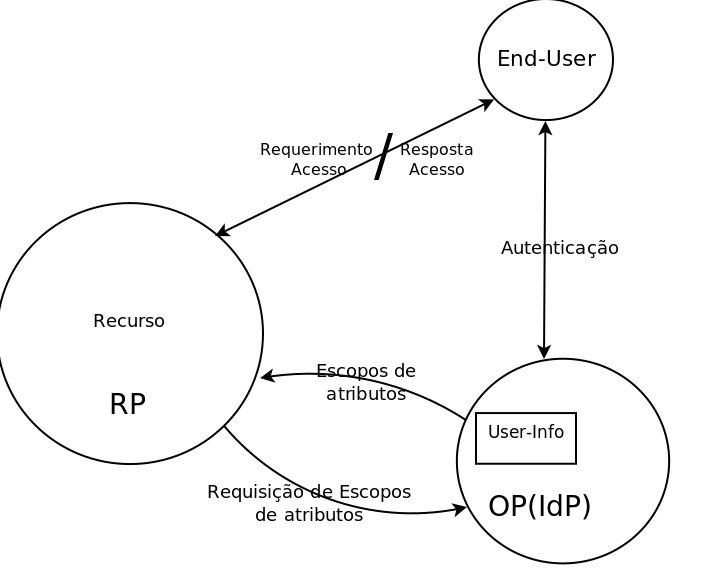
\includegraphics[height=5cm]{figuras/figura-proposta-especificacao-atual}
%		\label{Especificação atual do \textit{OpenID Connect}.}
%	}
%	\quad %espaco separador
%	\subfigure[Esquema geral da proposta]{
%		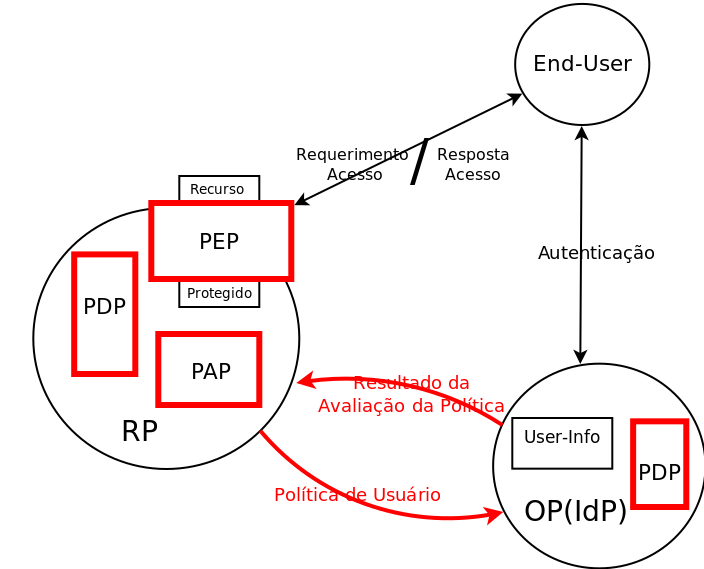
\includegraphics[height=5cm]{figuras/figura-proposta-modelo-proposto}
%		\label{Esquema geral da proposta do modelo.}
%	}
%	\caption{Esquemas demonstrando a especificação atual (à esquerda) e as modificações para acomodar a proposta do modelo.}
%	\label{fig-proposta-geral-colorido-subfiguras}
%\end{figure}


\section{Resultados esperados}\label{sec:result_esperados}

Para validar o modelo de autorização, mantendo a privacidade, será estabelecido um caso de uso, no qual serão criadas políticas de controle de acesso que atendam a maior parte dos requisitos. Como a avaliação de políticas pelos pontos de avaliação (PDP) já estão bem definidos, espera-se que a proposta possa ser validada sem problemas.

Em termos de desempenho, não há um trabalho relacionado que possa servir de parâmetro para quantificar o custo relativo da proposta. Mas, considerando que há necessidade de estender dois protocolos e incluir mais código de transporte, comunicação e avaliação de política, o desempenho tende a diminuir, aumentando a latência das decisões. Há duas questões que surgem para diminuir o impacto: a primeira seria a otimização, tanto dos códigos quanto das transações, isso após validar quanto à correção; a segunda, é considerar que essa proposta se destina a operações de controle de acesso que demandam intervenção humana na questão do consentimento, o que pode minorar a expectativa de latência nas respostas. O maior impacto poderia ocorrer no provedor de serviço, que poderia adotar soluções como otimização de avaliação de políticas de XACML \cite{mourad2014towards} e distribuição dos processos num ambiente paralelo.



\section{Validation of model}



\section{Conclusions}


This paper presents a new approach to realize fine-grained access control in environment with a identity provider OpenID Connect supplying PII data. The user controls the releasing the personal information. By adopting the evaluation of the service policies in the same domain of the identity provider, the personal data do not needs to be transported to the service provider. As a result of this, the privacy of PII is obtained and the user do not need care of the potential use of personal data by service providers. Important characteristic of this schema is the usability, because the user not need to established privacy policies concerning of manipulating his data.
Future works go in direction of research the monitoring and auditing of privacy protection provided by the IdP and on the other side there is the question of decomposition of policy and include this in the model presents in this paper.


\section*{Acknowledgements}
The authors would like to acknowledge the support from the LRG-UFSC.

\bibliographystyle{apsr}
\bibliography{bibliografia}


\end{document}
